\input{../preamb.tex}


\subtitle{Lecture 1}

\author{John Stachurski}

\date{June -- July 2022}


\begin{document}

\begin{frame}
  \titlepage
\end{frame}


\section{Introduction}


\begin{frame}
    \frametitle{Introduction}

    Lectures:

    \begin{itemize}
        \item Wednesday 13:00 -- 16:40  (in person, no zoom)
            \vspace{0.3em}
        \item Location: Seminar Room 515 (Economics building)
            \vspace{0.3em}
    \end{itemize}

            \vspace{0.3em}
            \vspace{0.3em}
    Lecturer: John Stachurski

    \begin{itemize}
        \item Email: \texttt{john.stachurski@anu.edu.au}
            \vspace{0.3em}
        \item Office: Daisuke Oyama's office (10th Floor)
            \vspace{0.3em}
        \item Office hours: Email me (for meeting times, not questions)
            \vspace{0.3em}
    \end{itemize}

\end{frame}




\begin{frame}
    \frametitle{Resources}

    \emp{Course homepage}: \url{https://github.com/jstac/tokyo_2022_coursework}

    \begin{itemize}
        \item please check regularly
    \end{itemize}

    \vspace{0.3em}
    \vspace{0.3em}
    \vspace{0.3em}
    \vspace{0.3em}

    \emp{Course notes}: \underline{Dynamic Programming Volume 1} 
                by John Stachurski and Thomas J.\ Sargent
    \vspace{0.3em}
    \vspace{0.3em}
    \vspace{0.3em}
    \vspace{0.3em}

    \begin{itemize}
        \item  Course notes will change! Print only small sections.
        \item Please help me fix typos / squash bugs
    \end{itemize}

    \vspace{0.3em}
    \vspace{0.3em}
    \vspace{0.3em}
    \vspace{0.3em}

    \emp{Programming resources} \url{https://lectures.quantecon.org/}
    
    \vspace{0.3em}
    \vspace{0.3em}
    \vspace{0.3em}
    \vspace{0.3em}


\end{frame}





\begin{frame}

    Supplementary reading:
    
    \begin{itemize}
        \item \emph{Abstract Dynamic Programming} by Dimitri Bertsekas, Athena
        Scientific, 2018
            \vspace{0.3em}
            \vspace{0.3em}
        \item \emph{Recursive Macroeconomic Theory} by Lars Ljungqvist and Thomas J. Sargent, MIT Press, 2018, chapters 1-7
            \vspace{0.3em}
            \vspace{0.3em}
        \item \emph{Recursive Methods in Dynamic Economics} by Nancy Stokey and Robert E. Lucas, Harvard University Press, 1989
            \vspace{0.3em}
            \vspace{0.3em}
        \item \emph{Introduction to Real Analysis} by Robert Bartle and Donald
            Sherbert, Wiley, 2011
            \vspace{0.3em}
            \vspace{0.3em}
        \item \emph{Analysis for Applied Mathematics} by Ward Cheney, Springer Science, 2013 
            \vspace{0.3em}
    \end{itemize}

\end{frame}




\section{Assessment}

\begin{frame}
    \frametitle{Assessment}
    
    \begin{enumerate}
        \item 40\% \navy{Programming Assignment} (details TBA)
            \vspace{0.4em}
            \begin{itemize}
                \item To be submitted as a Jupyter notebook
            \vspace{0.4em}
                \item Due date TBA
            \vspace{0.4em}
                \item Will include programming and analysis
            \end{itemize}
            \vspace{0.4em}
            \vspace{0.4em}
        \item 60\% \navy{Final Exam} (20/7/2022 1 pm)
            \vspace{0.4em}
            \begin{itemize}
                \item Analytical (no programming)
            \end{itemize}
    \end{enumerate}


\end{frame}





\section{Topics}

\begin{frame}
    \frametitle{Topics}

    \begin{itemize}
        \item Modern scientific computing
            \vspace{0.5em}
        \item Linear and nonlinear equations
            \vspace{0.5em}
        \item Markov chains
            \vspace{0.5em}
        \item Asset pricing
            \vspace{0.5em}
        \item Optimal stopping problems (job search, options, etc.)
            \vspace{0.5em}
        \item Markov control problems (savings, investment, inventories) 
            \vspace{0.5em}
        \item Recursive preferences
    \end{itemize}

\end{frame}


\section{Motivation}

\begin{frame}
    \frametitle{Motivation}

    Why do we need computers / computational methods?

    \vspace{1em}

    \Eg  A typical problem from \underline{undergraduate} choice theory:

    %
    \begin{equation}
        \max_{c_0, c_1} \left\{   u(c_0) + \beta u(c_1) \right\}
    \end{equation}
    %
    subject to 
    %
    \begin{equation}
       0 \leq c_0, c_1
       \quad \text{and} \quad
       c_1 \leq R(y_0 - c_0)
    \end{equation}
    %

            \vspace{0.5em}
            \vspace{0.5em}
    If $u' > 0, u'' < 0$ and $u'(0)=\infty$, then the unique
    solution obeys
    %
    \begin{equation*}
        u'(c_0) = \beta R u'(R(y_0 - c_0))
        \quad \text{and} \quad
       c_1 = R(y_0 - c_0)
    \end{equation*}
    %

\end{frame}

\begin{frame}

    In general, undergraduate style optimization problems are \emp{easy}

    \begin{itemize}
        \item All functions are differentiable
            \vspace{0.5em}
        \item Few choice variables (low dimensional)
            \vspace{0.51em}
        \item Concave (for max) or convex (for min)
            \vspace{0.51em}
        \item Interior solutions
            \vspace{0.51em}
        \item FOCs relatively simple
    \end{itemize}



\end{frame}




\begin{frame}
    
    But grad micro/macro and research problems are harder...
    \vspace{1em}

    \begin{itemize}
        \item High dimensions
            \vspace{0.6em}
        \item Nonsmooth functions
            \vspace{0.6em}
        \item Discrete choices
            \vspace{0.6em}
        \item Boundary solutions
            \vspace{0.6em}
        \item No analytical solution for FOCs
            \vspace{0.6em}
        \item Neither concave nor convex --- local maxima and minima
    \end{itemize}

            \vspace{0.6em}
            \vspace{0.6em}
    Most interesting research problems have these features

\end{frame}



\begin{frame}

    \Eg  Simple graduate macroeconomic problem:

            \vspace{0.5em}
    Choose consumption at time $t = 0, 1, \ldots$ to solve
    %
    \begin{equation}
        \label{eq:earnings}
        \EE \sum_{t=0}^{\infty} \beta^t u(c_t),
    \end{equation}
    %
    subject to 
    %
    \begin{equation}
        0 \leq a_{t+1} \leq R_t a_t + y_t - c_t
        \quad \text{and} \quad
        c_t \geq 0
        \qquad (t \geq 0)
    \end{equation}
    %

            \vspace{0.5em}
    Even for this simple problem,
    %
    \begin{itemize}
        \item Infinite dimensional because we choose $c_0, c_1, \ldots$
            \vspace{0.2em}
        \item Occasionally binding constraints
            \vspace{0.2em}
        \item No analytical solution
    \end{itemize}



\end{frame}


\begin{frame}
    \frametitle{Tools for this Course}

    We use two kinds of tools in this course

    \begin{enumerate}
        \item Programming / computation
            \vspace{1em}
        \item Mathematical analysis
    \end{enumerate}

        \vspace{1em}
        \vspace{1em}

    Let's talk a bit about them\ldots

\end{frame}



\section{Mathematics}

\begin{frame}
    \frametitle{Mathematical Background}

    We use three branches of mathematics in this course:

    \begin{enumerate}
        \item Linear algebra 
            \vspace{0.5em}
        \item Real analysis
            \vspace{0.5em}
        \item Probability theory
    \end{enumerate}

\end{frame}


\begin{frame}
    \frametitle{Linear algebra and Analysis}
    
    For solving equations and optimization problems

    What is/are the solution/solutions to these equations?

    \begin{enumerate}
        \item $x = a x + b$
            \vspace{0.5em}
        \item $x = x + 1$
            \vspace{0.5em}
        \item $x^2 = 1$
    \end{enumerate}

    \pause
    \vspace{0.5em}
    \vspace{0.5em}

    Now let $x$ be $n \times 1$ and $A$ be $n \times n$

    When does this \navy{vector equation} have a unique solution ?  

    \begin{equation*}
        A x = b
    \end{equation*}
    
\end{frame}


\begin{frame}
    
    When does this vector equation in $\RR^n$ have a unique solution?
    %
    \begin{equation*}
        x = A x + b
    \end{equation*}

    \pause
    \vspace{0.5em}
    When is the solution given by 
    %
    \begin{equation*}
        x = (I - A)^{-1} b ?
    \end{equation*}

    \vspace{0.5em}
    \vspace{0.5em}


    \pause
    When does the \navy{method of successive approximations} converge?

    \begin{enumerate}
        \item pick any $x_0 \in \RR^n$
            \vspace{0.4em}
        \item set $x_{n+1} = A x_n + b$ for $n = 0, 1, \ldots$
    \end{enumerate}


\end{frame}


\begin{frame}
    
    Now let's make it a bit harder:

    \begin{equation*}
        x = ((Ax)^{1/\gamma} + b)^\gamma,
        \qquad \gamma > 0
    \end{equation*}


    \vspace{0.5em}
    \vspace{0.5em}

    When does this have a solution?
    \vspace{0.5em}

    Is it unique?
    \vspace{0.5em}

    How would we compute it?

\end{frame}


\begin{frame}
    \frametitle{Probability}

    This sequence is {\sc iid}


    \begin{figure}
       \begin{center}
           \scalebox{.5}{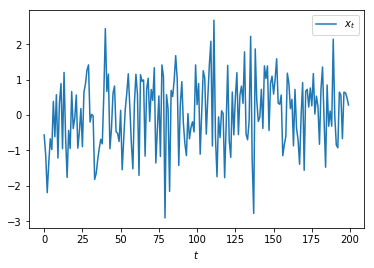
\includegraphics{sp1.png}}
       \end{center}
    \end{figure}

\end{frame}



\begin{frame}

    Does it follow that, for some function $h$, we have

    \begin{equation}
        \frac{1}{n} \sum_{t=1}^n h(X_t) \to \EE h(X_t)
        \;\; ?
    \end{equation}

        \vspace{0.5em}
    If so this is good:

    \begin{itemize}
        \item Right hand side is something we want to compute
        \vspace{0.5em}
        \item Left hand side is simulated from the model
        \vspace{0.5em}
        \item Convergence means we can use Monte Carlo\ldots
    \end{itemize}

\end{frame}


\begin{frame}

    This sequence is \emp{not} {\sc iid}


    \begin{figure}
       \begin{center}
           \scalebox{.5}{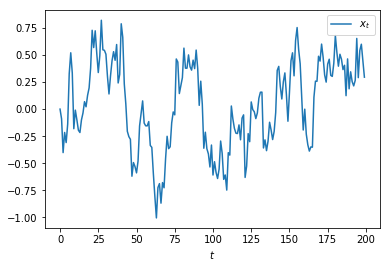
\includegraphics{sp2.png}}
       \end{center}
    \end{figure}


\end{frame}



\begin{frame}

    Is it possible that, for some function $h$, we have

    \begin{equation}
        \frac{1}{n} \sum_{t=1}^n h(X_t) \to \EE h(X_t)
        \;\; ?
    \end{equation}


    \vspace{2em}

    What conditions do we require?

\end{frame}


\section{Programming}


\begin{frame}
    \frametitle{Programming Background --- Hardware}

    CPU frequency (clock speed) growth is slowing

    \begin{figure}
       \begin{center}
        \scalebox{.22}{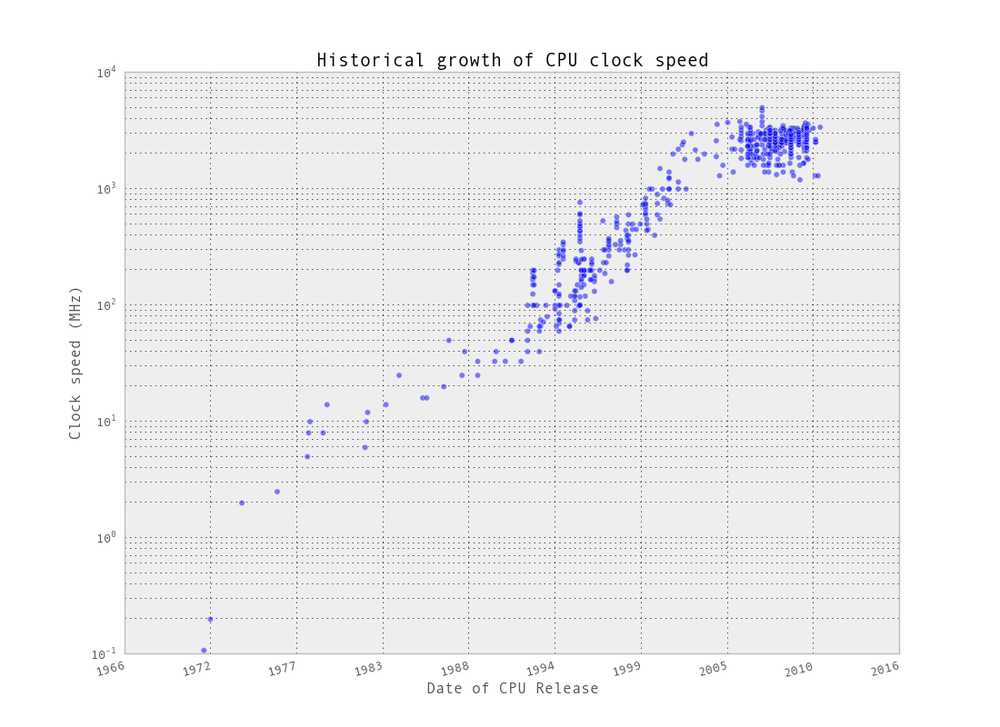
\includegraphics{processor_clock.png}}
       \end{center}
    \end{figure}

\end{frame}


\begin{frame}
    
    Chip makers have responded by developing multi-core processors

    \begin{figure}
       \begin{center}
        \scalebox{.22}{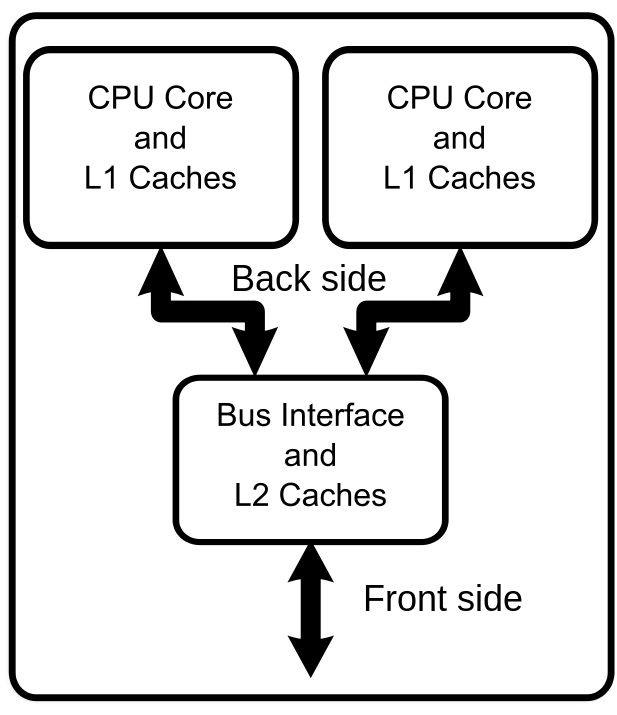
\includegraphics{dual_core.png}}
       \end{center}
    \end{figure}

    Source: Wikipedia


\end{frame}


\begin{frame}
    
    and GPUs...

    \begin{figure}
       \begin{center}
           \scalebox{.4}{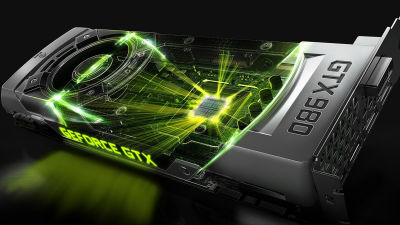
\includegraphics{gpu.jpg}}
       \end{center}
    \end{figure}


\end{frame}



\begin{frame}

    Issues
    %
    \begin{itemize}
        \item Exploiting multiple cores / threads is nontrivial
            \vspace{0.5em}
            \vspace{0.5em}
        \item Sometimes we need to redesign algorithms
            \vspace{0.5em}
            \vspace{0.5em}
        \item Sometimes we can use tools that automate exploitation of multiple cores
    \end{itemize}

\end{frame}




\begin{frame}
    \frametitle{Programming}

    The assignment will require programming

            \vspace{0.5em}
            \vspace{0.5em}

    Acceptable languages

    \begin{itemize}
        \item Python
            \vspace{0.5em}
        \item Julia
    \end{itemize}

            \vspace{0.5em}
            \vspace{0.5em}
            \vspace{0.5em}
    We will use a mix

    \begin{itemize}
        \item Mainly Python in class
            \vspace{0.5em}
        \item Julia used in the textbook
    \end{itemize}


\end{frame}






\begin{frame}
    \frametitle{Programming Background}
    
    A common classification:
    %
    \begin{itemize}
        \item \emp{low} level languages (assembly, C, Fortran)
            \vspace{0.5em}
        \item \emp{high} level languages (Python, Ruby, Haskell)
    \end{itemize}

    \vspace{0.5em}
    \vspace{0.5em}
    \vspace{0.5em}
    \vspace{0.5em}
    \vspace{0.5em}
    \navy{Low level languages} give us fine grained control 


\end{frame}





\begin{frame}[fragile]
    
    \Eg $1 + 1$ in assembly

    {\small
    \begin{minted}{as}
pushq   %rbp
movq    %rsp, %rbp
movl    $1, -12(%rbp)
movl    $1, -8(%rbp)
movl    -12(%rbp), %edx
movl    -8(%rbp), %eax
addl    %edx, %eax
movl    %eax, -4(%rbp)
movl    -4(%rbp), %eax
popq    %rbp
    \end{minted}
    }



\end{frame}


\begin{frame}
    
    \navy{High level languages} give us abstraction, automation, etc.

\end{frame}



\begin{frame}[fragile]

    \Eg Reading from a file in Python
    
    \begin{minted}{python}
    data_file = open("data.txt")
    for line in data_file:
        print(line.capitalize()) 
    data_file.close()
    \end{minted}

\end{frame}






\begin{frame}

    Jane Street on readability:

    \vspace{0.5em}
    \vspace{0.5em}
    
    \begin{quote}
        There is no faster way for a
        trading firm to destroy itself than to deploy a piece of trading
    software that makes a bad decision over and over in a tight loop.
        \vspace{2em}

        Part of Jane Street's reaction to these technological risks was to
        put a very strong focus on building software that was easily
    understood---software that was readable.
        \vspace{2em}

        -- {\sf Yaron Minsky, Jane Street}
    \end{quote}


\end{frame}





\begin{frame}
    \frametitle{Trade-Offs}

    \begin{figure}
       \begin{center}
        \scalebox{.36}{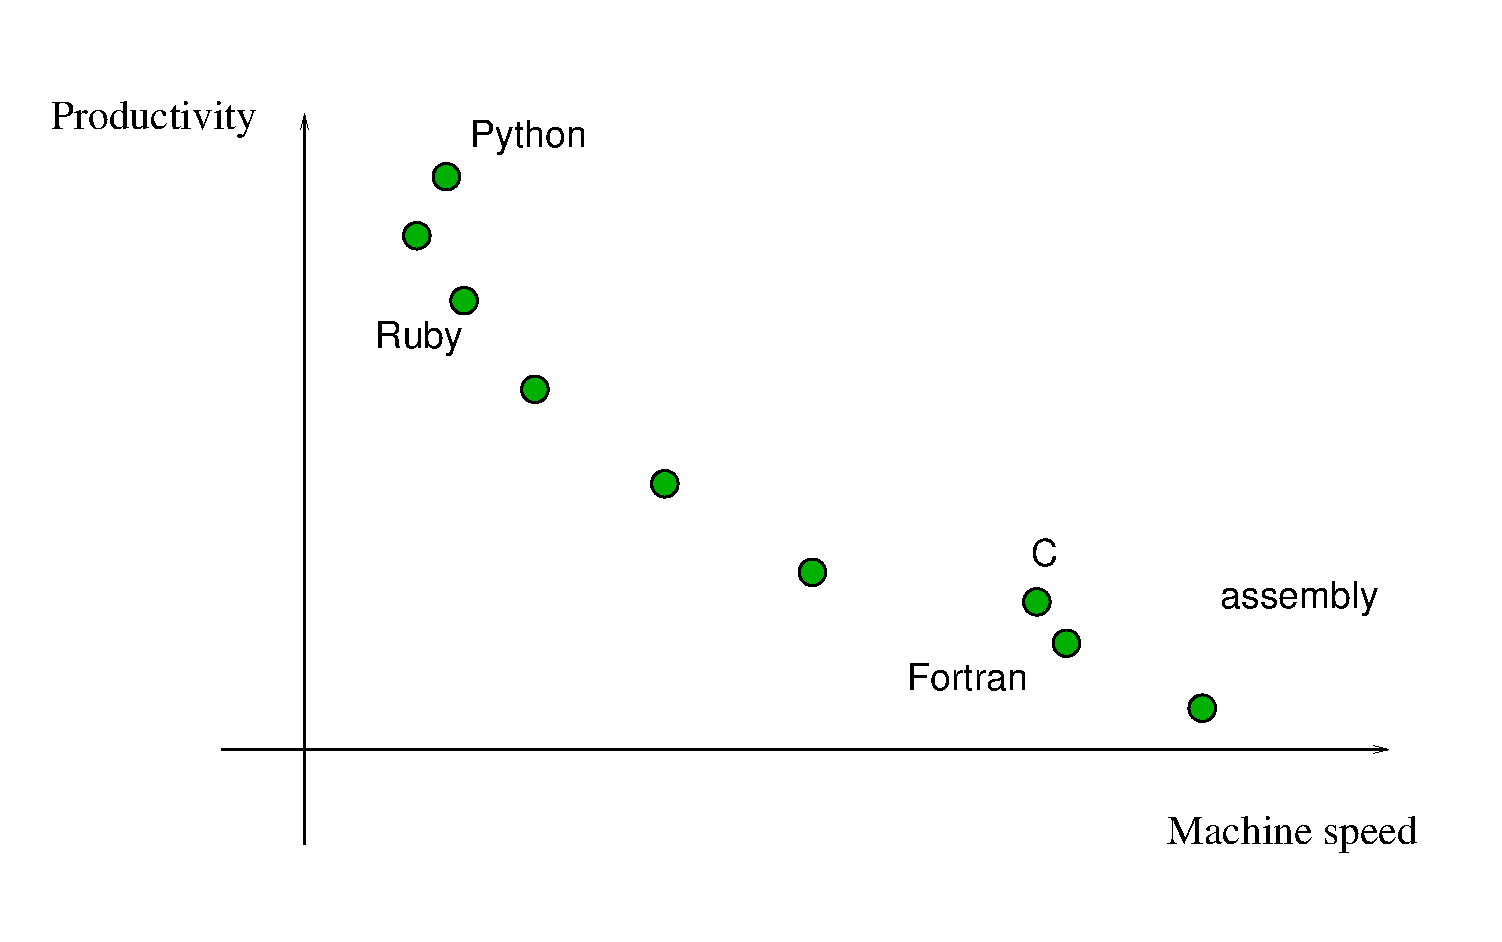
\includegraphics{tradeoff.pdf}}
       \end{center}
    \end{figure}

\end{frame}



\begin{frame}[fragile]
    \frametitle{But what about scientific computing?}
    
    \navy{Requirements}

    \begin{itemize}
        \item \underline{Productive} --- easy to read, write, debug, explore
            \vspace{0.4em}
            \vspace{0.4em}
            \vspace{0.4em}
        \item \underline{Fast} computations
    \end{itemize}

\end{frame}




\begin{frame}
    \frametitle{Trade-Offs}

    \begin{figure}
       \begin{center}
        \scalebox{.36}{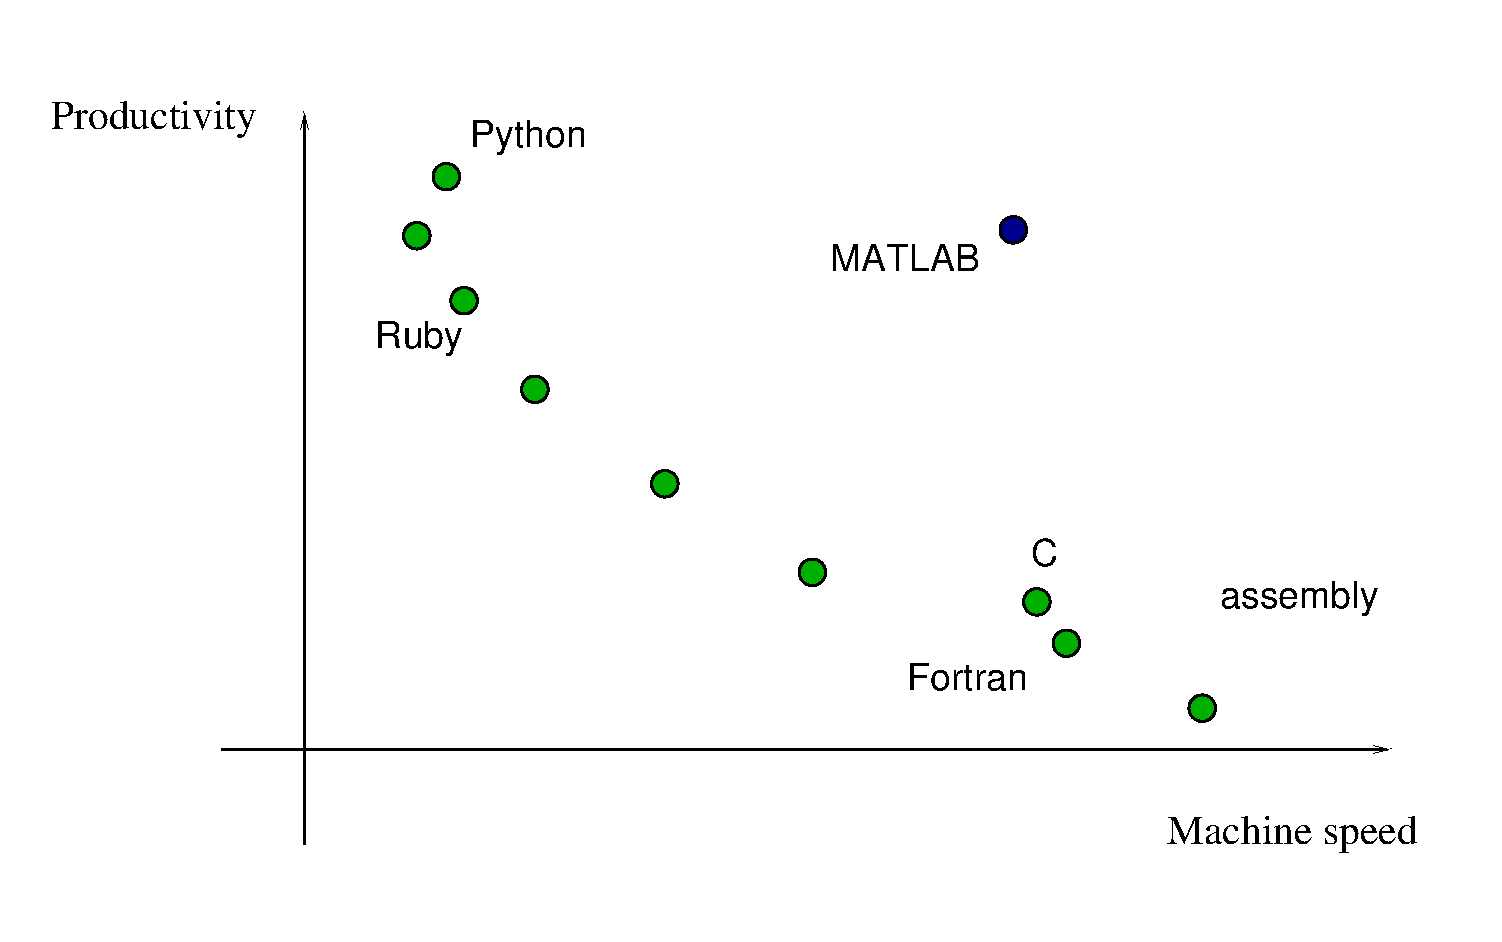
\includegraphics{tradeoff2.pdf}}
       \end{center}
    \end{figure}

\end{frame}


\begin{frame}
    \frametitle{Trade-Offs}

    \begin{figure}
       \begin{center}
        \scalebox{.36}{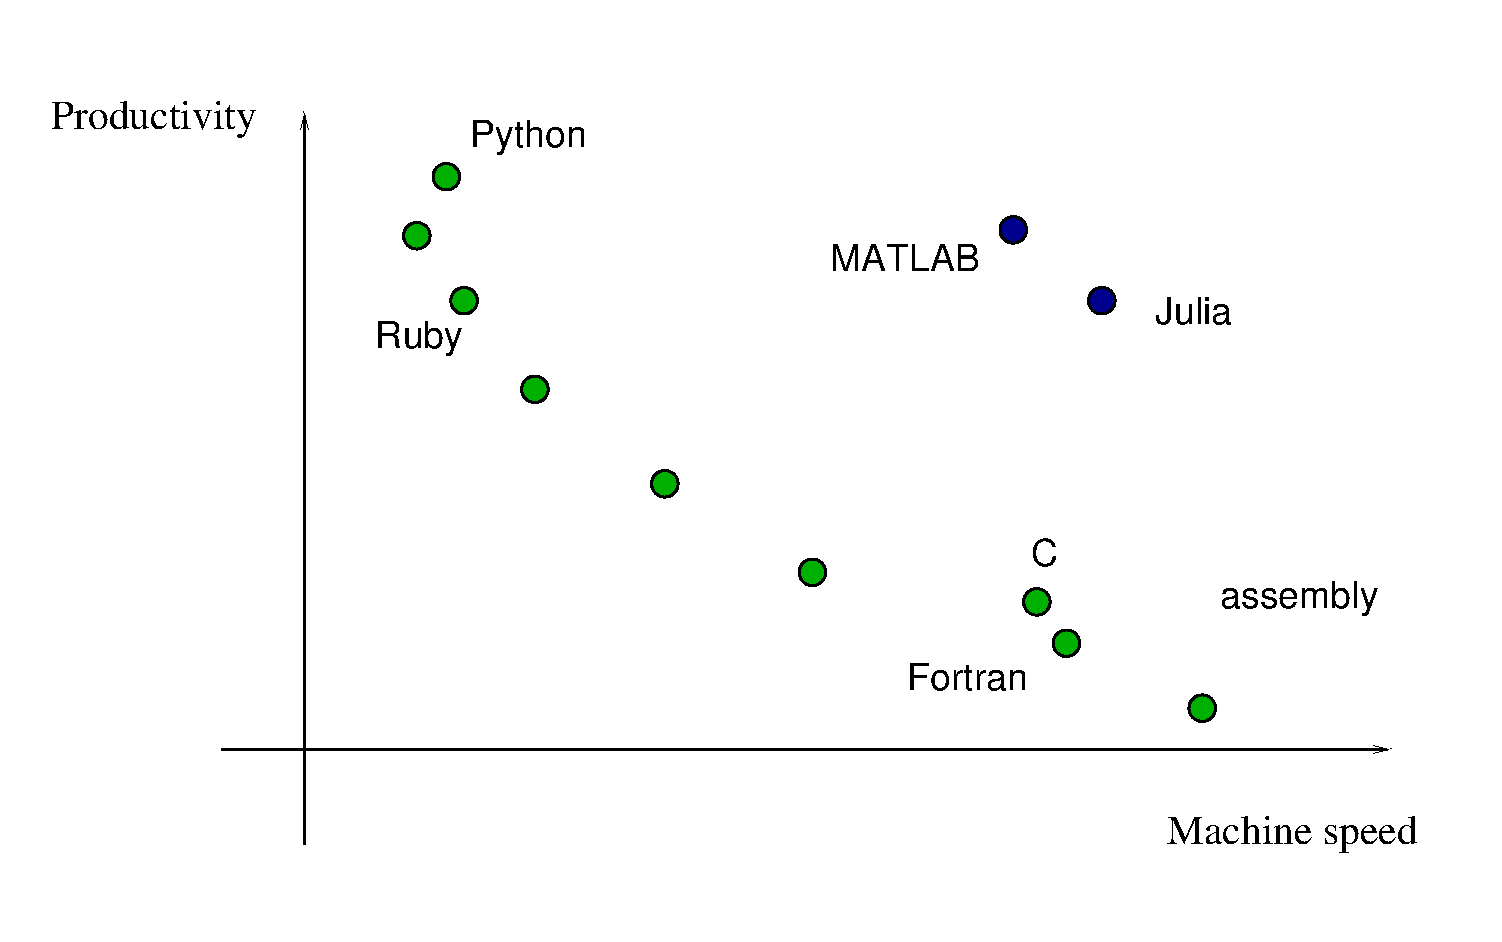
\includegraphics{tradeoff3.pdf}}
       \end{center}
    \end{figure}

\end{frame}


\begin{frame}
    \frametitle{Trade-Offs}

    \begin{figure}
       \begin{center}
        \scalebox{.36}{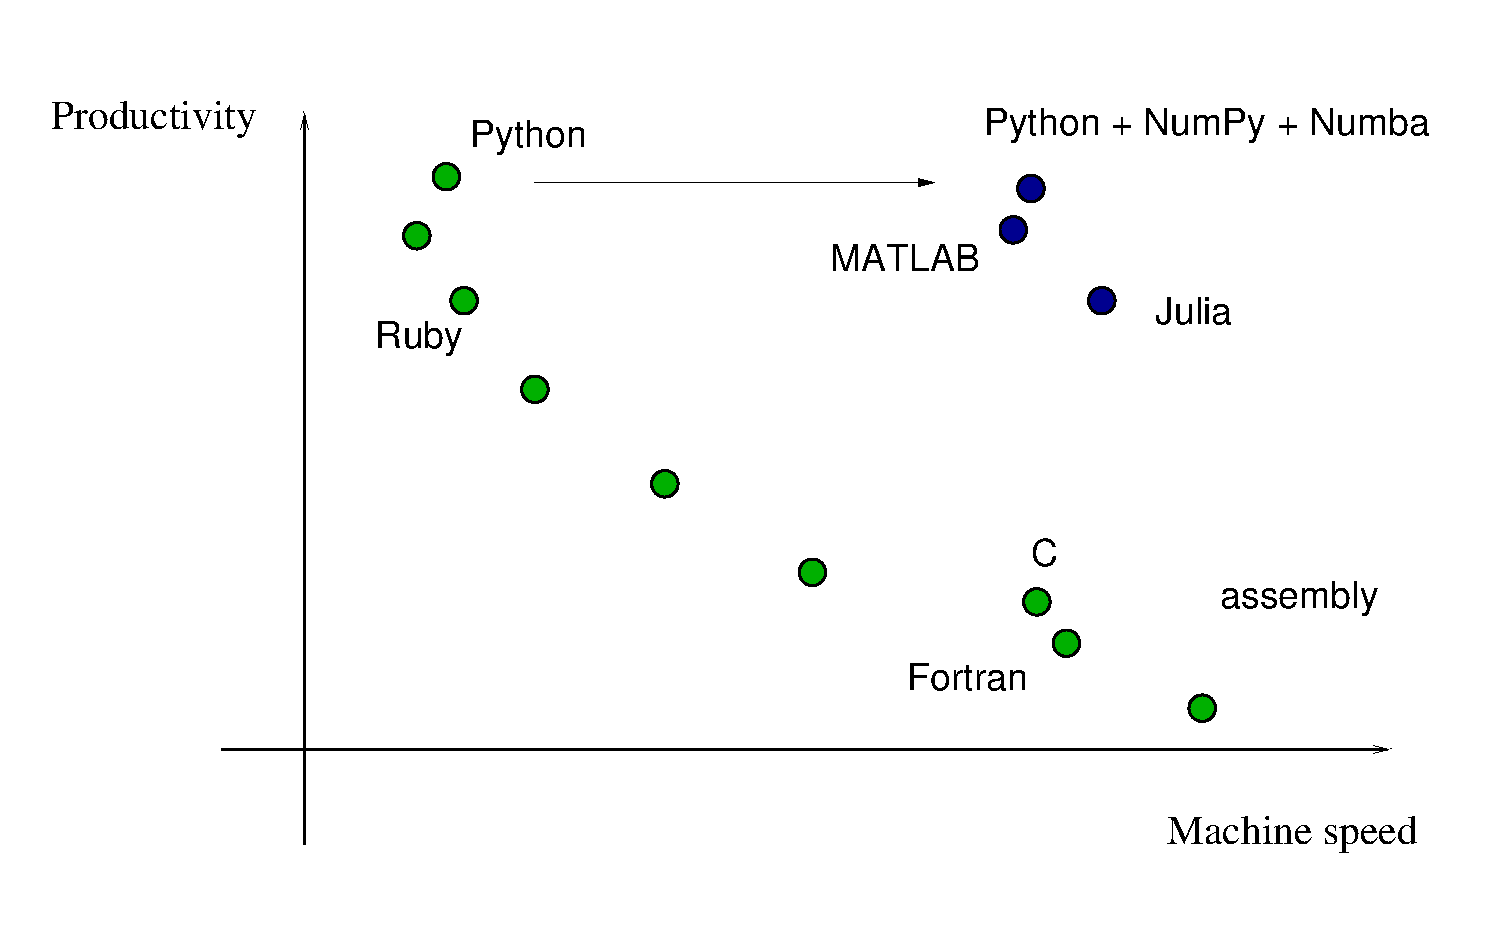
\includegraphics{tradeoff4.pdf}}
       \end{center}
    \end{figure}

\end{frame}

\begin{frame}
    \frametitle{Key Takeaways}

    \begin{itemize}
        \item \underline{Don't} write in C / C++ / Fortran, no matter what your professor says
            \vspace{0.4em}
            \vspace{0.4em}
        \item JIT compilation is changing scientific computing
            \vspace{0.4em}
            \vspace{0.4em}
        \item Same with parallelization
            \vspace{0.4em}
            \vspace{0.4em}
        \item New algorithms, new techniques --- and opportunities
    \end{itemize}

\end{frame}


\begin{frame}
    \frametitle{Demo: Fast Computing with Python}

    Let's quickly see what a difference computing platforms make

            \vspace{0.4em}
    \begin{enumerate}
        \item Downloand the notebook from \url{https://notes.quantecon.org/submission/622ed4daf57192000f918c61}
            \vspace{0.4em}
        \item Run on \url{colab.research.google.com}
    \end{enumerate} 
            \vspace{0.4em}
            \vspace{0.4em}

    Notes:
    %
    \begin{itemize}
        \item You need a Google account
            \vspace{0.4em}
        \item Runs faster if you have Colab Pro
    \end{itemize}

\end{frame}




\section{Need for Analysis}

\begin{frame}
    \frametitle{Need for Analysis}

    The demonstration showed the power of modern hardware/software

    \vspace{1em}

    But \navy{can faster computers always save us}?

    \vspace{0.5em}
    If so, do we really need to care about clever maths/algorithms?

    \vspace{0.5em}
    Below we demonstrate that
    %
    \begin{itemize}
        \item Fast computers are \underline{not enough}
        \vspace{0.5em}
        \item Clever algorithms and analysis are vital!
    \end{itemize}

    The demonstration concerns \emp{brute force} maximization

\end{frame}




\begin{frame}
    
    \begin{figure}
       \begin{center}
           \scalebox{.4}{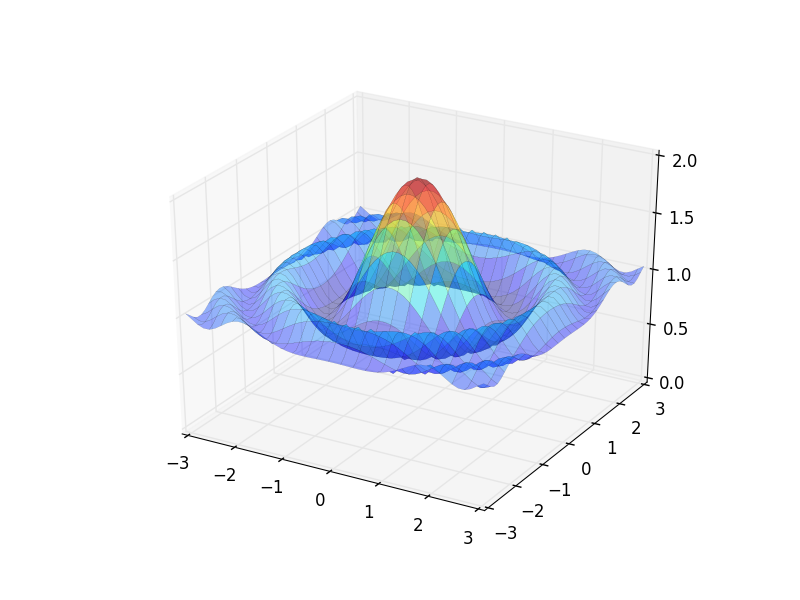
\includegraphics{brute_force_1.png}}
           \caption{The function to maximize}
       \end{center}
    \end{figure}

\end{frame}



\begin{frame}
    
    \begin{figure}
       \begin{center}
           \scalebox{.4}{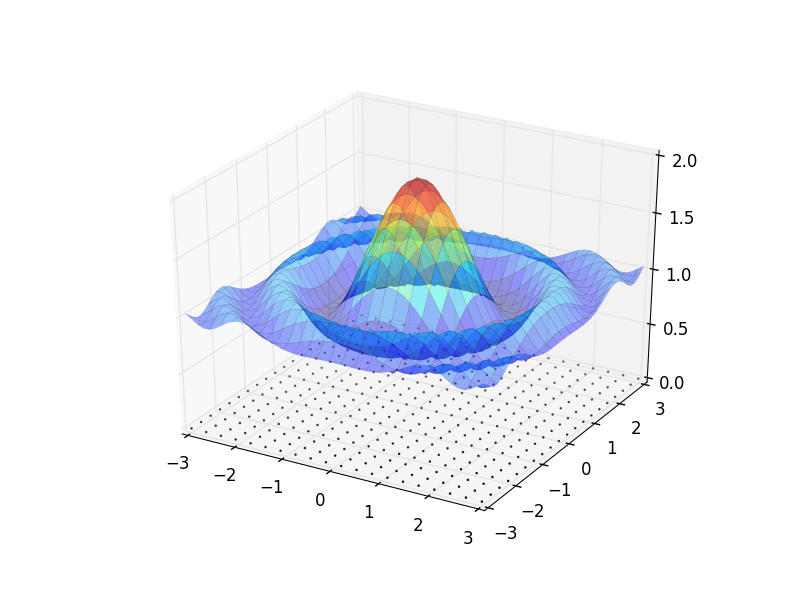
\includegraphics{brute_force_2.png}}
           \caption{Grid of points to evaluate the function at}
       \end{center}
    \end{figure}

\end{frame}

\begin{frame}
    
    \begin{figure}
       \begin{center}
           \scalebox{.4}{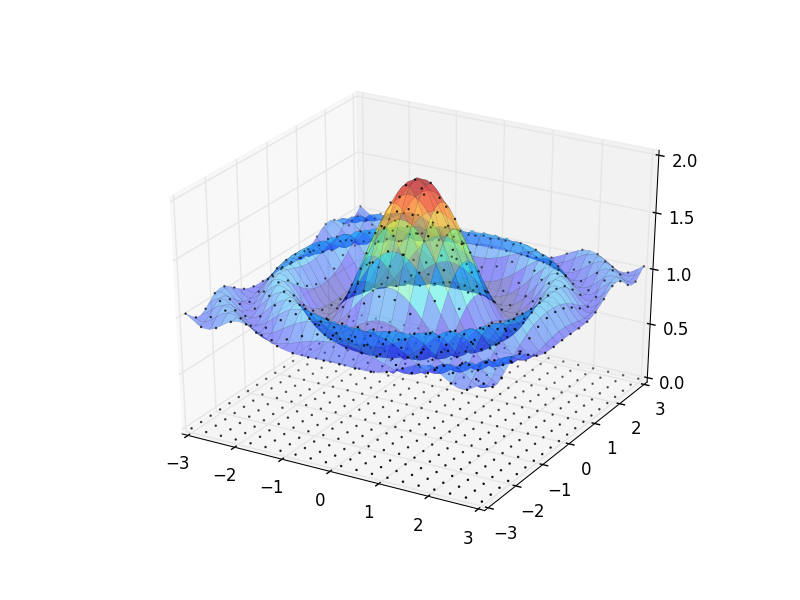
\includegraphics{brute_force_3.png}}
           \caption{Evaluations}
       \end{center}
    \end{figure}

\end{frame}


\begin{frame}
    
    Grid size = $20 \times 20 = 400$

    Outcomes

    \begin{itemize}
        \item Number of function evaluations $= 400$
        \item Time taken = almost zero 
        \item Maximal value recorded $= 1.951$
        \item True maximum $= 2$
    \end{itemize}

    Not bad and we can easily do better

\end{frame}


\begin{frame}
    
    \begin{figure}
       \begin{center}
           \scalebox{.4}{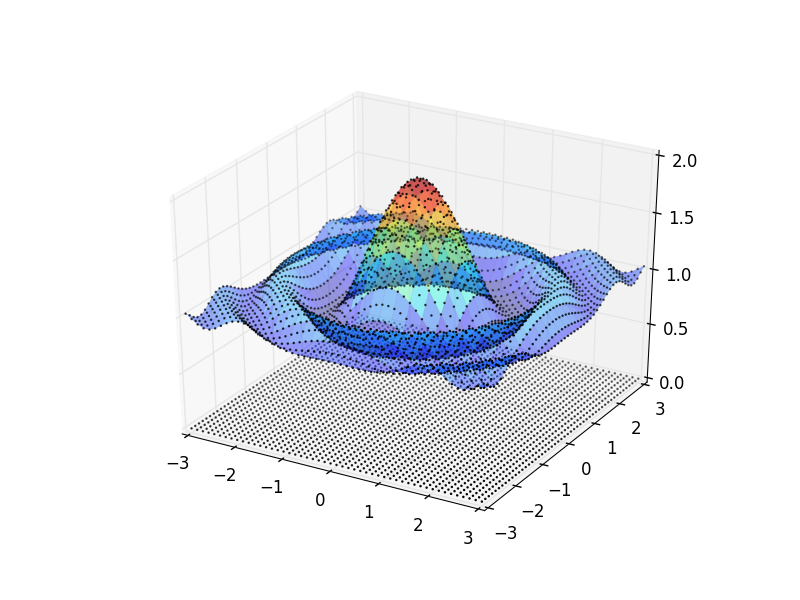
\includegraphics{brute_force_4.png}}
           \caption{$50^2 = 2500$ evaluations}
       \end{center}
    \end{figure}

\end{frame}


\begin{frame}
    
    \begin{itemize}
        \item Number of function evaluations $= 50^2$
        \item Time taken = $400$ $\mu$s
        \item Maximal value recorded $= 1.992$
        \item True maximum $= 2$
    \end{itemize}

    \vspace{1em}

    So why even study optimization?

\end{frame}


\begin{frame}
    
    The problem is mainly with larger numbers of choice variables

    \begin{itemize}
        \item 3 vars: $\max_{x_1, x_2, x_3} f(x_1, x_2, x_3)$
        \item 4 vars: $\max_{x_1, x_2, x_3, x_4} f(x_1, x_2, x_3, x_4)$
        \item $\cdots$
    \end{itemize}

    If we have 50 grid points per variable and 
    
    \begin{itemize}
        \item 2 variables then evaluations $=50^2 = 2500$
        \item 3 variables then evaluations $=50^3 = 125,000$
        \item 4 variables then evaluations $=50^4 = 6,250,000$
        \item 5 variables then evaluations $=50^5 = 312,500,000$
        \item $\cdots$
    \end{itemize}

\end{frame}


\begin{frame}
    
    \Eg Recent study: Optimal placement of drinks across vending machines in
    Tokyo

    Approximate dimensions of problem:

    \begin{itemize}
        \item Number of choices for each variable $=2$
        \item Number of choice variables $=1000$
    \end{itemize}

    Hence number of possibilities $=2^{1000}$

    \vspace{1em}

    How big is that?

\end{frame}


\begin{frame}[fragile]
    
\begin{pythoncode}
In [10]: 2**1000
Out[10]:
107150860718626732094842504906000181056140481170
553360744375038837035105112493612249319837881569
585812759467291755314682518714528569231404359845
775746985748039345677748242309854210746050623711
418779541821530464749835819412673987675591655439
460770629145711964776865421676604298316526243868
37205668069376
\end{pythoncode}

\end{frame}


\begin{frame}[fragile]

    Let's say my machine can evaluate about 1 billion possibilities per second

    How long would that take?

\end{frame}


\begin{frame}[fragile]


\begin{pythoncode}
In [16]: (2**1000 / 10**9) / 31556926  # In years
Out[16]:
339547840365144349278007955863635707280678989995
899349462539661933596146571733926965255861364854
060286985707326991591901311029244639453805988092
045933072657455119924381235072941549332310199388
301571394569707026437986448403352049168514244509
939816790601568621661265174170019913588941596
\end{pythoncode}

\end{frame}



\begin{frame}[fragile]

    What about high performance computing?
    
    \begin{itemize}
        \item more powerful hardware
        \item faster CPUs
        \item GPUs
        \item vector processors
        \item cloud computing
        \item massively parallel supercomputers
        \item $\cdots$
    \end{itemize}

    Let's say speed up is $10^{12}$ (wildly optimistic)



\end{frame}

\begin{frame}[fragile]


\begin{pythoncode}
In [19]: (2**1000 / 10**(9 + 12)) / 31556926
Out[19]:
3395478403651443492780079558636357072806789899958
9934946253966193359614657173392696525586136485406
0286985707326991591901311029244639453805988092045
9330726574551199243812350729415493323101993883015
7139456970702643798644840335204916851424450993981
6790601568621661265174170019
\end{pythoncode}

    For comparison:

\begin{pythoncode}
In [20]: 5 * 10**9 # Expected lifespan of sun
Out[20]: 5000000000
\end{pythoncode}


\end{frame}



\begin{frame}
    \frametitle{Summary}

    Software, platforms and hardware \navy{do} matter
    %
    \begin{itemize}
        \item Fast machine code
            \vspace{0.5em}
        \item Compiler optimization tricks
            \vspace{0.5em}
        \item Parallelization (CPUs, GPUs)
    \end{itemize}

    \vspace{2em}

    But algorithms matter even more


    \begin{itemize}
        \item Clever ideas reduce curse of dimensionality
            \vspace{0.5em}
        \item Mathematical analysis is needed to find and study algorithms
    \end{itemize}


\end{frame}


\section{Programming tools}


\begin{frame}
    \frametitle{Getting Started with Python}

    Option 1: Install locally

        \vspace{0.5em}

    \begin{enumerate}
        \item Go to \url{anaconda.com}
            \vspace{0.5em}
        \item Download Anaconda Python
            \vspace{0.5em}
        \item Install
            \vspace{0.5em}
        \item Start \navy{Jupyter notebook}
    \end{enumerate}

            \vspace{0.5em}
    Option 2:
    %
    \begin{enumerate}
        \item Get a Google account (if necessary)
        \item Go to \url{https://colab.research.google.com}
    \end{enumerate}

\end{frame}

\begin{frame}
    \frametitle{Getting Started with Python}

    Get notebooks from 

    \begin{center}
        \url{https://github.com/jstac/tokyo_2022_coursework/tree/main/lecture_1}
    \end{center}


    Steps:
    %
    \begin{enumerate}
        \item Download the notebooks to your machine 
            \vspace{0.5em}
            \begin{itemize}
                \item One by one (raw), zip file, clone
            \end{itemize}
            \vspace{0.5em}
        \item Go to Jupyter Notebook landing page (dashboard)
            \vspace{0.5em}
        \item Click on \emp{Upload}
            \vspace{0.5em}
        \item (or in Colab, use \texttt{File -> Upload notebook})
    \end{enumerate}

\end{frame}


\begin{frame}
    \frametitle{Homework}

    \begin{enumerate}
        \item Review what we have covered!
            \vspace{0.5em}
        \item Optionally, start to read Chapter 1 of \underline{Dynamic Programming}
    \end{enumerate}

\end{frame}




\end{document}
